\documentclass{standalone}
\begin{document}

\subsection{Implementación de unidad gráfica}

\paragraph{}
Para la implementación del motor de juego que es nuestro objetivo, esta sección explica la implementación de su primer componente que es un motor gráfico que facilite el despliegue de imágenes en haskell.

\paragraph{}
La librería de despliegue gráfico seleccionada para el proyecto es OpenGL, que es una librería que interactúa con el GPU para brindar despliegue grafico acelerado por hardware. OpenGL tiene la ventaja de ser multiplataforma e independiente del sistema de ventanas y del sistema operativo en que corra la aplicación, permitiendo así a nuestra aplicación ser fácilmente portable entre diferentes dispositivos.

\paragraph{}
La interfaz de OpenGL para haskell es un binding de la librería escrita en c, haciendo necesario el uso de apuntadores e IO para poder interactuar con el contexto de OpenGL, siendo el objetivo de este módulo facilitar el despliegue gráfico, es importante hacer una librería que exponga una interfaz más funcional (de la misma forma en la que el monad IO oculta la naturaleza imperativa del mundo exterior) que sea más familiar a los usuarios de lenguajes funcionales y también que la librería provea de facilidades para cargar recursos multimedia al contexto de OpenGL así como controlar el proceso de despliegue gráfico.

\paragraph{}
El primer paso para usar OpenGL es la creación del contexto, para ello se ha elegido la librería GLUT, que es una librería de utilidades para aplicaciones que utilicen OpenGL, enfocándose primariamente en I/O a nivel de sistema operativo, operaciones como la creación y control de ventanas y entrada del teclado.

\paragraph{}
Trabajos realizados con GLUT se encuentran en el módulo EasyGLUT. La primera necesidad a la hora de usar GLUT está en definir callbacks para los diferentes eventos, entrada de mouse y teclado y cambios en el estado de la ventana. La librería provee funciones que inicializan una ventana GLUT (y consigo el contexto de OpenGL) y se definen diversos callbacks para el contexto de GLUT que procesan la entrada de la ventana y se acumula toda la entrada para ser procesada en el ciclo principal del programa.

\paragraph{}
El siguiente paso es facilitar el uso de GLUT dentro del ciclo principal de ejecución. Visto desde un punto de vista funcional, se puede considerar a GLUT como  un conjunto de cómputos que definen y controlan el estado de la ventana GLUT, así, estos cómputos pueden ser visto como un monad \cite{moggi1991notions} \cite{wiki:MonadsComputation} \cite{wiki:MonadsContainers}, que dentro de lenguajes funcionales facilitaría la interacción del usuario con la librería, ocultando apuntadores y demás detalles de comunicación de la librería con GLUT. De esta forma se introduce el monad GLUT que tiene las propiedades de poder ser consultado por eventos externos y entrada de dispositivos además de poder controlar una ventana de despliegue y un contexto de OpenGL. Con este monad es innecesario correr una función peligrosa de tipo IO como ciclo principal de la aplicación, sino que podemos correr una función de tipo GLUT en la cual se puede garantizar el correcto uso del estado global que representa el contexto de GLUT gracias a las restricciones y garantías del monad.

\paragraph{}
Ahora que se ha trabajado el contexto de OpenGL se necesita facilitar la carga de recursos multimedia. La librería EasyGL en sus submodulos ofrece funciones para cargar texturas en formatos PNG,Bitmap, Jpeg, Radiance, Tiff y Gif que son cargadas directamente al GPU como objetos de OpenGL con facilidades para especificar el tipo de filtrado y clamping. También se ofrece facilidades para cargar mayas poligonales en formato obj, al GPU para despliegue, con un conjunto de representaciones intermedias que permiten manipular estas mayas (como agregarle la normal a las caras en caso que no tengan).

\paragraph{}
El módulo EasyGL.Shader provee facilidades para cargar y compilar archivos de shaders a OpenGL. Todos los shaders compilados con esta librería poseerán atributos adicionales que reciben la posición del vértice, junto con su normal y coordenada de textura, facilitando la comunicación entre aplicación y shaders. Adicionalmente se creó el monad Uniform que representa las acciones de cargar datos a los atributos de los shaders, que combinado con una clase Uniform, ayuda a garantizar que solo datos que puedan ser aceptados por el GPU sean cargados a este.

\paragraph{}
El siguiente ejemplo muestra el código de una aplicación que cargar y muestra un mayado con un shader dado en un color dado por la aplicación al shader:

\begin{lstlisting}
import EasyGL
import EasyGLUT
import System.Exit
import System.IO (stderr)
import Control.Monad.IO.Class (MonadIO,liftIO)
import qualified Graphics.Rendering.OpenGL as GL

armadillo :: Shader -> IO (Material,Entity)
armadillo myShader = do
  m <- makeMaterial myShader []
  case m of
    Left s -> putStrLn s >> exitFailure
    Right mat -> do
      e <- readObj2Ent "./armadillo.obj"
      return (mat,e)

main = do
	-- se inicializa el contexto de OpenGL y GLUT.
  initOpenGLEnvironment 800 600 "test"
	-- se carga los shaders.
  myShader <-
		loadShadersFromFile
			["./vertex.shader","./frag.shader"]
			[VertexShader,FragmentShader]
			(Just stderr)
	-- se carga el mayado.
  assets <- armadillo myShader
  initGL $ myfun assets

  -- funcion para el ciclo principal de la aplicacion.
myfun :: (Material,Entity) -> GLUT ()
myfun (mat,ent) = do
	liftIO $ GL.preservingMatrix $ do
		useCamera cam
		drawWithMat mat ent $
			set "color" $ GL.Color4 1 1 0 (1 :: GL.GLfloat)
	where
		(Right cam) =
			createCamera3D 0.0 0.0 10.0 0 0 0 30 (800/600) 0.3 200
\end{lstlisting}

\begin{figure}[h!]
  \caption{Captura de pantalla 1.}
  \begin{center}
    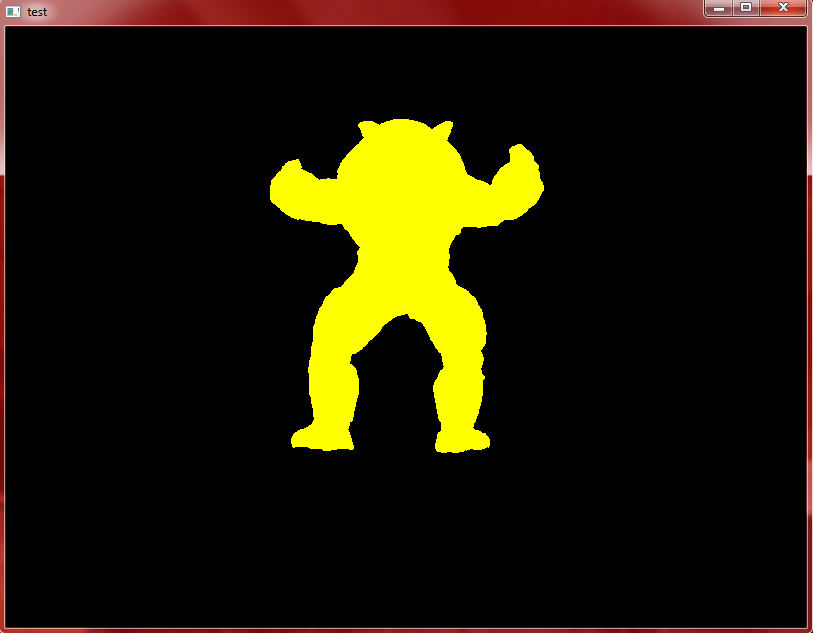
\includegraphics[width=0.8\textwidth]{sceenshot1}
  \end{center}
\end{figure}

\subsection{Implementación de entidades y motor lógico}

\paragraph{}
Las implementaciones actuales de motores de juegos, como es el caso de por ejemplo Unity, implementan la lógica del juego en un sistema entidad-componente, en el cual todos los objetos que viven en una escena están representados como una entidad, que a su vez consiste de uno o más componentes que añaden diferentes funcionalidades y comportamientos \cite{JasonGregory-GameEngineArchitecture}. Este sistema es usado en motores que usan lenguajes orientados a objetos ya que elimina ambigüedad en la jerarquía de herencia de las clases, que son difíciles de entender, mantener o extender.

\paragraph{}
Este sistema, sin embargo, tiene sus problemas como lo son la comunicación entre componentes y los sistemas que administran dichos componentes y el costo que se incurre al tener que iterar por los diferentes componentes de cada entidad.

\paragraph{}
Este diseño podría ser implementado en lenguajes funciones como haskell definiendo un tipo de dato que englobe a los componentes y haciendo entidades compuestas de listas (u otra estructura) de componentes, y funcionaria, pero sería difícil de escalar a largo plazo y costoso por la naturaleza de datos inmutables de programación funcional, además de los problemas nativos del sistema entidad-componente. La solución más aceptada para este problema en lenguajes funcionales es el uso de FRP, donde los objetos están definidos en base a funciones tiempo dependientes (comportamientos) que pueden ser compuestas y combinadas. Este esquema es mucho más atractivo y compatible con el enfoque en funciones puras y composición de la programación funcional. Gerold Meisinger hace en su devblog una explicación más detallada de porque cambiar el sistema entidad-componente por FRP \cite{devblog:Meisinger}.

\paragraph{}
Para el uso de FRP se usa la librería Yampa por tener una documentación más extensa así como una librería más completa que librerías similares.

\paragraph{}
Para implementar la lógica del juego bajo el esquema FRP es necesario poder crear objetos que dependan solo del tiempo y de la entrada que los usuarios generen, generando como salida la información necesaria para que los módulos que se encarguen de labores especificas del motor de juego pueden realizar las acciones correspondientes. En cuanto a la dependencia del tiempo, una señal de función (SF) de Yampa hace en trabajo, pero para mantener esta función pura es necesario establecer una entrada específica, es así que definimos un objeto como:

\begin{lstlisting}
type Object outState eventType =
  SF (ObjInput outState eventType) (ObjOutput outState eventType)
\end{lstlisting}

\paragraph{}
Donde outState es un tipo de dato de salida de los objetos que es la única salida que otros objetos serán capases de observar, y eventType es un tipo de dato que indica los diferentes eventos ocurridos por la interacción de diferentes objetos. Así, un objeto es una SF que recibe la entrada del mundo exterior, la salida de los objetos de la iteración anterior y los eventos que se generen, y genera como salida un conjunto de datos que indica al motor diferentes acciones IO a realizar, como desplegar una maya poligonal, y la salida outState que deben de generar los objetos.

\paragraph{}
Siguiendo el ejemplo de The Yampa Arcade, una escena de juego debe estar compuesta de una colección de objetos que sea actualizada en el tiempo, para la implementación de esta colleccion se implementa en el módulo Val.Strict.IL el tipo de dato IL (Identity List), que es una estructura capaz de almacenar objetos de un mismo tipo e identificarlos con un id único, esta capacidad de identificar únicamente a los objetos es importante para que otros objetos puedan buscar información de otro objeto especifico, como un jugador que aterriza sobre una plataforma, el jugador debe moverse junto con la plataforma con la que colisiono, no con cualquier otra. Esta estructura IL está representada en la librería como un mapa de id a elemento, se eligió un mapa ya que la implementación en haskell tiene muy buen costo amortizado para agregar y eliminar (O (log n)), la otra opción era un arreglo, pero como los id no son consistentes con la posición en el arreglo, los costos de eliminar era alto (O n) y al agregar un elemento se podría tener que extender el arreglo, también costoso.

\paragraph{}
Ya que el proceso de actualización de los objetos en cada frame es puro, implementando la clase Traversable de haskell a nuestra estructura IL, la librería Control.Parallel.Strategies nos permite calcular la actualización de los diferentes objetos en paralelo aprovechando la mayor cantidad de procesadores disponibles.

\paragraph{}
El modulo Val.Strict.Data implementa ObjInput y ObjOutput.

\begin{lstlisting}
data ObjInput state eventType = ObjInput {
  oiEvents :: Event eventType,
  oiGameInput :: GameInput,
  oiPastFrame :: IL state
}
\end{lstlisting}

\paragraph{}
ObjInput permite a los objetos recibir eventos generados con la interacción de otros objetos, la entrada generada por el usuario y el estado de salida generado en el frame anterior por todos los objetos.

\begin{lstlisting}
data ObjOutput state eventType = ObjOutput {
  ooObjState :: !state,
  ooRenderer :: Maybe (ResourceIdentifier,Transform,Uniform ()),
  ooKillReq :: Event (),
  ooSpawnReq :: Event [Object state eventType],
  ooWorldReq :: [IOReq eventType], -- request to perform IO
  ooWorldSpawn :: [IO ()],
  ooUIReq :: [UIActions]
}
\end{lstlisting}

\paragraph{}
ObjOutput representa la salida que deben de generar los objetos, ooObjState representa la salida que otros objetos podrán ver, ooRenderer indica al sistema para desplegar un objeto en OpenGL, ooKillReq es un pedido al sistema para eliminar el objeto actual, ooSpawnReq permite crear un objeto nuevo, finalmente, el rento de los campos de ObjOutput permiten generar diferentes tipos de funciones asíncronas en IO (como leer un archivo), cuyo resultado será dado al objeto cuando terminen.

\paragraph{}
El ciclo principal que corre una escena de juego corre en 3 hilos de cómputo que son creados durante la inicialización del programa.

\paragraph{Hilo 1, hilo lógico}
Este hilo se caracteriza por actualizar la colección de objetos cada frame, este hilo inicia recibiendo la entrada del usuario del hilo 2 y el retorno de las funciones asíncronas generadas por los objetos manejados por el hilo 3. Con estos dos datos se actualizan los objetos en base al tiempo transcurrido y la salida de ellos es transmitida a los otros hilos.

\paragraph{Hilo 2, hilo de despliegue}
Este hilo maneja el contexto de OpenGL y GLUT, incia enviando la entrada del usuario al hilo 1 y recibe la salida de los objetos generados en el hilo 1. Con esta salida se puede generar el despliegue de gráficos.

\paragraph{Hilo 3, hilo de IO}
Este hilo existe para que los objetos del juego puedan ejecutar funciones IO de manera asíncrona. Este hilo mantiene una lista de todas las funciones asíncronas en corrida. Este hilo inicia evaluando la culminación de alguna función y enviando los resultados al hilo 1, luego recibe la salida del hilo 1 y corre cualquier nueva función asíncrona que los objetos soliciten.

\paragraph{}
Si bien se tiene 3 hilos principales, hay que recalcar que el hilo 1 actualiza los objetos en paralelo y el hilo 3 corre las funciones asíncronas cada una en un hilo, por lo que se hace el máximo uso posible del procesador.

\subsection{Ejemplo de uso del motor}

\paragraph{}
El siguiente ejemplo muestra una escena con 200 esferas que se mueven en una dirección y se mueven en la dirección contraria si colisionan o llegan al límite de un área.

\begin{lstlisting}
{-# LANGUAGE Arrows #-}

import Val.Strict hiding (yaw)
import EasyGL
import EasyGLUT
import Data.Either
import System.IO (stderr)
import FRP.Yampa hiding (RandomGen,randomR)
import Data.List (find)
import System.Random
import qualified Graphics.Rendering.OpenGL as GL
import qualified Data.Map as Map
import qualified System.Random.TF as TF

-- Se cargan los recursos a utilizar en el ejemplo
load :: IO ResourceMap
load = do
  myShader <- loadShadersFromFile
    ["./assets/3Dshaders/vertex.shader",
    "./assets/3Dshaders/ColorShader.shader"]
    [VertexShader,FragmentShader]
    (Just stderr)
  (Right mat) <- makeMaterial myShader []
  let plane = ("plane","./assets/plane.obj",mat)

  myShader <- loadShadersFromFile
    ["./assets/3Dshaders/vertex.shader",
    "./assets/3Dshaders/NormalShader.shader"]
    [VertexShader,FragmentShader]
    (Just stderr)
  (Right mat) <- makeMaterial myShader []
  let sphere = ("sphere","./assets/sphere.obj",mat)

  loadResouces [plane,sphere]

-- Informacion de los objetos.
data GameState = Null
  | Sphere {
    x :: Double,
    y :: Double,
    z :: Double,
    size :: Double
  }

collition :: GameState -> GameState -> Bool
collition Sphere{x=x1,z=y1} Sphere{x=x2,z=y2} =
  ( (x1-x2)^2 + (y1-y2)^2 ) < 4
collition _ _ = False

data EventTypes = Collition GameState
  | NoCollition

instance MergeableEvent EventTypes where
  union NoCollition NoCollition = NoCollition
  union a NoCollition = a
  union NoCollition a = a
  union a b = a

-- Funcion que detecta colisiones.
collitionGen :: IL GameState -> IL (Event EventTypes)
collitionGen inObjs = mapILWithKey aux inObjs
  where
    assocs = assocsIL inObjs
    aux key obj = case valid of
      (x:_) -> Event $ Collition . snd $ x
      [] -> noEvent
      where
        valid = filter
          (\(key2,obj2) -> key /= key2 && collition obj obj2 )
          assocs

cam :: SF (GameInput,IL GameState) Camera3D
cam = proc _ -> do
    returnA -< c
    where
    (Right c) = createCamera3D 0 150 0 0 (-90) 0 30 (800/600) 0.3 200

plane :: Object GameState EventTypes
plane = proc _ -> do
  let ret = newObjOutput Null
      trans = Transform
        (GL.Vector3 0 (-1) 0)
        (Quaternion 0 (GL.Vector3 0 1 0))
        2 1 2
      uni = do
        set "color" $ GL.Color4 1 1 1 (1 :: GL.GLfloat)
  returnA -< ret{ooRenderer=Just("plane",trans,uni)}

moveSF :: GL.GLdouble
  -> GL.GLdouble
  -> (GL.GLdouble,GL.GLdouble)
  -> SF () (GL.GLdouble,GL.GLdouble)
moveSF limMax limMin d@(dir,_) =
  if (dir > 0) then aux2 (> limMax) (< limMin) d else aux2 (< limMin) (> limMax) d
  where
    aux2 f1 f2 (dir,initx) = switch (aux f1 dir initx) (aux2 f2 f1)
    aux f dir initx = proc _ -> do
      xnew <- (+initx) ^<< integral -< dir
      e <- edge -< f xnew
      returnA -< ((xnew,dir),tag e (-dir,xnew))

moveXZSF :: GL.GLdouble -> GL.GLdouble -> (GL.GLdouble,GL.GLdouble) ->
  GL.GLdouble -> GL.GLdouble -> (GL.GLdouble,GL.GLdouble) ->
  SF a (GL.GLdouble,GL.GLdouble,GL.GLdouble,GL.GLdouble)
moveXZSF limMaxX limMinX initX limMaxZ limMinZ initZ = proc _ -> do
  (x,dirx) <- moveSF limMaxX limMinX initX -< ()
  (z,dirz) <- moveSF limMaxZ limMinZ initZ -< ()
  returnA -< (x,z,dirx,dirz)

type Info = (GL.GLdouble,GL.GLdouble,GL.GLdouble,GL.GLdouble)

getCollition :: SF (ObjInput GameState EventTypes,Info) (Event Info)
getCollition = proc (oi,salida) -> do
  let myEvent = event noEvent toEvent $ inputEvent oi
  returnA -< tag myEvent salida
  where
    toEvent NoCollition = noEvent
    toEvent a = Event a

sphere :: GL.GLdouble -> GL.GLdouble
  -> GL.GLdouble -> GL.GLdouble
  -> Object GameState EventTypes
sphere initx initz velx velz = proc gi -> do
  rec
    rot <- impulseIntegral -< (180,tag e (-360))
    e <- iPre noEvent <<< edge -< rot > 360
    (x,z,dirx,dirz) <- moveArr (initx,initz,velx,velz) -< gi

  let ret = newObjOutput $ Sphere (realToFrac x) 0 (realToFrac z) 1
      trans = Transform
        (GL.Vector3 x 0 z)
        (Quaternion rot (GL.Vector3 0 1 0))
        1 1 1
  returnA -< ret{ooRenderer=Just("sphere",trans,return ())}
  where
    moveArr (x,z,velx,velz) = dkSwitch
      (moveXZSF 40 (-40) (velx,x) 40 (-40) (velz,z))
      (getCollition >>> notYet)
      (\sf (x,z,velx,velz) -> moveArr (x,z,-velx,-velz) )

randomSphere :: RandomGen g => g -> (Object GameState EventTypes, g)
randomSphere g = (sphere initx initz velx velz,g4)
  where
    (initx,g1) = randomR (-39,39) g
    (initz,g2) = randomR (-39,39) g1
    (velx,g3) = randomR (-4,4) g2
    (velz,g4) = randomR (-4,4) g3

randomSphereList :: RandomGen g => g -> [Object GameState EventTypes]
randomSphereList g = obj:(randomSphereList g1)
	where
		(obj,g1) = randomSphere g

main :: IO ()
main = do
  gen <- TF.mkSeedTime >>= return . TF.seedTFGen
  let il = [plane]++(take 200 $ randomSphereList gen)
  initScenePar cam load [collitionGen] il

\end{lstlisting}

\begin{figure}[h!]
  \caption{Captura de pantalla 2.}
  \begin{center}
    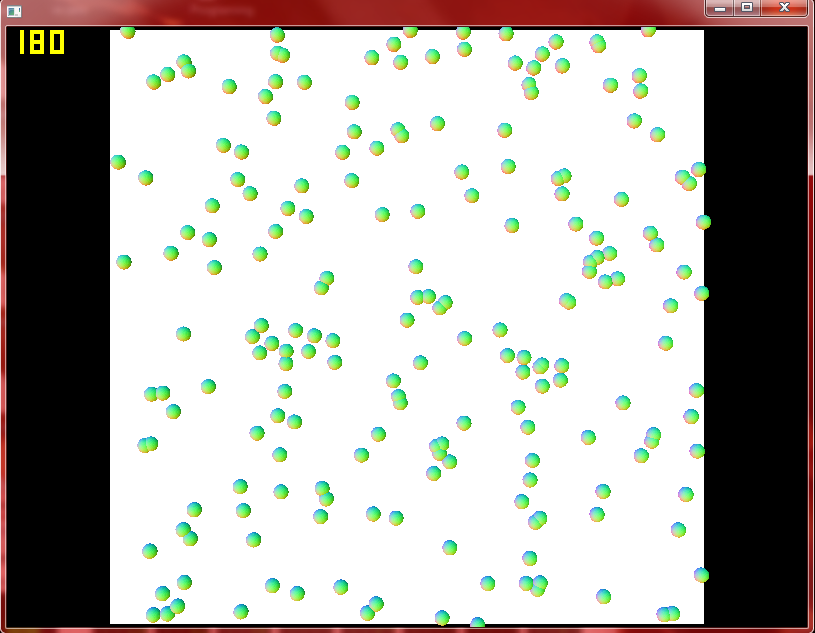
\includegraphics[width=0.8\textwidth]{screenshot2}
  \end{center}
\end{figure}

\paragraph{}
Este ejemplo muestra una forma en la que se puede construir una escena con objetos que interactúan entre sí con poco código. Este programa puede aprovechar la concurrencia del procesador solo con ser compilado con opciones especiales.

\paragraph{}
Usando el programa FRAPS en Windows, es posible medir los FPS o frames per second de la aplicación. Corriendo la aplicación varias veces en una misma computadora con 1, 2, 3 y 4 hilos, se optiene que los FPS promedio son de 115, 132, 171 y 176 respectivamente.


\end{document}
